\documentclass{beamer}

\newcommand{\course}{CS 1331 Introduction to Object Oriented Programming}
\newcommand{\lesson}{Binary Trees}
\newcommand{\code}{http://www.cc.gatech.edu/~simpkins/teaching/gatech/cs1331/code}

\author[Chris Simpkins] 
{Christopher Simpkins \\\texttt{chris.simpkins@gatech.edu}}
\institute[Georgia Tech] % (optional, but mostly needed)

\date[CS 1331]{}

\subject{\lesson}


% If you have a file called "university-logo-filename.xxx", where xxx
% is a graphic format that can be processed by latex or pdflatex,
% resp., then you can add a logo as follows:

% \pgfdeclareimage[width=0.6in]{coc-logo}{cc_2012_logo}
% \logo{\pgfuseimage{coc-logo}}

\mode<presentation>
{
  \usetheme{Berlin}
  \useoutertheme{infolines}

  % or ...

 \setbeamercovered{transparent}
  % or whatever (possibly just delete it)
}

\usepackage{hyperref}
\usepackage{fancybox}
\usepackage{listings}
\usepackage[abbr]{harvard}

\usepackage[english]{babel}
% or whatever

\usepackage[utf8]{inputenc}
% or whatever

\usepackage{times}
\usepackage[T1]{fontenc}
% Or whatever. Note that the encoding and the font should match. If T1
% does not look nice, try deleting the line with the fontenc.


\usepackage{listings}
 
% "define" Scala
\lstdefinelanguage{scala}{
  morekeywords={abstract,case,catch,class,def,%
    do,else,extends,false,final,finally,%
    for,if,implicit,import,match,mixin,%
    new,null,object,override,package,%
    private,protected,requires,return,sealed,%
    super,this,throw,trait,true,try,%
    type,val,var,while,with,yield},
  otherkeywords={=>,<-,<\%,<:,>:,\#,@},
  sensitive=true,
  morecomment=[l]{//},
  morecomment=[n]{/*}{*/},
  morestring=[b]",
  morestring=[b]',
  morestring=[b]""",
}

\usepackage{color}
\definecolor{dkgreen}{rgb}{0,0.6,0}
\definecolor{gray}{rgb}{0.5,0.5,0.5}
\definecolor{mauve}{rgb}{0.58,0,0.82}
 
% Default settings for code listings
\lstset{frame=tb,
  language=scala,
  aboveskip=2mm,
  belowskip=2mm,
  showstringspaces=false,
  columns=flexible,
  basicstyle={\scriptsize\ttfamily},
  numbers=none,
  numberstyle=\tiny\color{gray},
  keywordstyle=\color{blue},
  commentstyle=\color{dkgreen},
  stringstyle=\color{mauve},
  frame=single,
  breaklines=true,
  breakatwhitespace=true,
  keepspaces=true
  %tabsize=3
}


\title[\course] % (optional, use only with long
                                      % paper titles)
{\lesson}

\subtitle{}
%% {Include Only If Paper Has a Subtitle}

\newcommand{\link}[2]{\href{#1}{\textcolor{blue}{\underline{#2}}}}


% If you wish to uncover everything in a step-wise fashion, uncomment
% the following command: 

% \beamerdefaultoverlayspecification{<+->}


\begin{document}

\begin{frame}
  \titlepage
\end{frame}

%------------------------------------------------------------------------
\begin{frame}[fragile]{Binary Trees}


\begin{itemize}
\item Binary Tree Nodes
\item Binary Search Trees
\item Iterators
\end{itemize}


\end{frame}
%------------------------------------------------------------------------



%------------------------------------------------------------------------
\begin{frame}[fragile]{Binary Tree Nodes}


The nodes of a binary tree have
\begin{itemize}
\item a data item,
\item a link to a left node, and
\item a link to a right node.
\end{itemize}

\begin{lstlisting}[language=Java]
    private class Node<E> {
        E item;
        Node<E> left;
        Node<E> right;
        
        Node(E item, Node<E> left, Node<E> right) {
            this.item = item;
            this.left = left;
            this.right = right;
        }
    }
\end{lstlisting}

Just as in the other linked data structures we've studied, binary trees are recursive.


\end{frame}
%------------------------------------------------------------------------

%------------------------------------------------------------------------
\begin{frame}[fragile]{Binary Tree Structure}



\begin{itemize}
\item Every tree has a distinguished {\it root node} with no parent.
\begin{itemize}
\item All other nodes have exactly one parent.
\end{itemize}
\item Nodes which have no children are called {\it leaf nodes}.
\item Nodes which have children are called {\it interior nodes}.
\item Every node has 0, 1, or 2 children.
\item Every node can be reached by a unique path from the root node.
\end{itemize}

\begin{center}
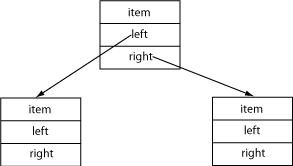
\includegraphics[height=1.25in]{binary-tree.png}
\end{center}


\end{frame}
%------------------------------------------------------------------------

%------------------------------------------------------------------------
\begin{frame}[fragile]{Binary Search Trees}


A binary search tree (BST) is a binary tree in which for any node,  
\begin{itemize}
\item all the elements in the node's left subtree are less than the node's data item, and
\item all the elements in the node's right subtree are equal to or greater than the node's data item.
\end{itemize}

A BST is distinguished by this property, but it's ADT is simple: add elements, find element's in the tree, and iterate over the elements in a tree.


\end{frame}
%------------------------------------------------------------------------

%------------------------------------------------------------------------
\begin{frame}[fragile]{Maintaining The BST Property}


To add a new value to binary tree and maintain the BST property, we  
\begin{itemize}
\item insert new nodes for data items into the left subtree of a node if the new item is less than the node's item, or
\item the right subtree otherwise.
\end{itemize}
Every new item creates a leaf node, which can later become an interior node after additional items have been added. Here's the structure of a BST after adding the sequence of numbers 3, 4, 1, 5, 2:
\vspace{-.05in}
\begin{center}
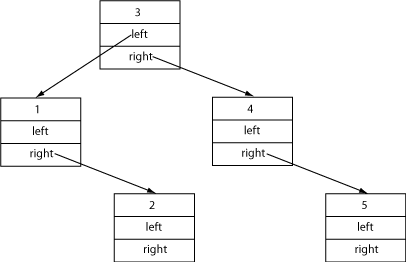
\includegraphics[height=1.5in]{binary-tree-nums.png}
\end{center}

\end{frame}
%------------------------------------------------------------------------

%------------------------------------------------------------------------
\begin{frame}[fragile]{Traversing a Binary Tree}


There are three primary ways to traverse a binary tree:

Pre-order:
\begin{itemize}
\item Process node's item.
\item Process left subtree.
\item Process right subtree.
\end{itemize}

In-order:
\begin{itemize}
\item Process left subtree.
\item Process node's item.
\item Process right subtree.
\end{itemize}

Post-order:
\begin{itemize}
\item Process left subtree.
\item Process right subtree.
\item Process node's item.
\end{itemize}

There are variations on these strategies.

\end{frame}
%------------------------------------------------------------------------

%------------------------------------------------------------------------
\begin{frame}[fragile]{Iterators}


Iterators can free clients from implementing such traversal algorithms.  We can even plug our data structures into Java's for-each loop by implementing {\tt java.lang.Iterable}:
\begin{lstlisting}[language=Java]
public interface Iterable<T> {
    java.util.Iterator<T> iterator();
}
\end{lstlisting}
As a reminder, {\tt java.util.Iterator}:
\begin{lstlisting}[language=Java]
public interface Iterator<E> {
    boolean hasNext();

    E next();

    void remove();
}
\end{lstlisting}

Let's implement an in-order iterator for a binary tree, a non-trivial task, to get an appreciation for the value of pre-defined iterators.

\end{frame}
%------------------------------------------------------------------------


% %------------------------------------------------------------------------
% \begin{frame}[fragile]{}


% \begin{lstlisting}[language=Java]

% \end{lstlisting}

% \begin{itemize}
% \item
% \end{itemize}


% \end{frame}
% %------------------------------------------------------------------------



\end{document}
